\chapter{3. Control Strategy}

The objective of this chapter is to present the control strategy used in the PEV, based on the Direct Tilt Control (DTC). First, the lateral stability of the vehicle is studied, in order to understand the different strategies for lateral control. Then, the dynamic model is transformed into an space state model, much more easy to work with in control theory. Finally, the theory behind Linear Quadratic Regulator (LQR) and the Regulator Problem with Internal Stability (RPIS) is explained and the control gains are calculated.

\section{Stability Study}
\begin{marginfigure}[10cm]
	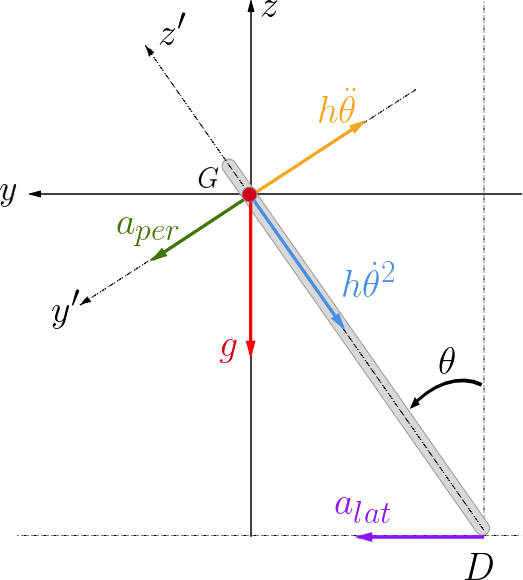
\includegraphics[width=1.2\linewidth]{figs/03/yz2}
	\caption{Forces acting on the center of gravity}
	\label{yz2}
\end{marginfigure}
\subsubsection{\textbf{Lateral Acceleration}}

The lateral acceleration $a_{lat}$ denotes the normal acceleration induced by the curvilinear motion of the vehicle, measured in the plane $XY$ at ground level at point D (Figure \ref{yz2}), and directed towards the center of rotation of the trajectory.
\[a_{lat}=\ddot{y}+V_{x}\dot{\psi}\]
Therefore, $a_{lat}$ is a function of the yaw rate (and hence the steering angle) and the longitudinal speed imposed by the driver. It is independent of the vertical position (angle of inclination) of the chassis.

\subsubsection{\textbf{Perceived Lateral Acceleration}}

In the frame reference $y',z'$, the acceleration at the point G decomposes into $a_{per}$ in the $y'$ direction and into $a_{z}$ in the $z'$ direction. The perceived lateral acceleration $a_{per}$ is the result of the accelerations at the center of gravity of the vehicle along the $y'$. 
\begin{equation}
a_{per}=a_{lat}\cos\theta+h\ddot{\theta}-g\sin\theta
\label{a_per}
\end{equation}
The objective for the control of lateral stabilization of the vehicle and the comfort of the driver will be to impose $a_{per}=0$. The vehicle is in lateral equilibrium if the perceived lateral acceleration is zero, i.e. $a_{per}=0$ (\textbf{sufficient condition for lateral stability})\cite[-2cm]{mourad:tel-00787310}.
\newpage
The fact that $a_{per}$ depends on $a_{lat}$ and $\theta$, implies that it depends on the trajectory, on the longitudinal velocity, and on the angle of inclination. However, the angle of inclination $\theta$ will be the key variable to ensure stability. We define by $\theta_{des}$ the desired position of $\theta$ which ensures $a_{per}=0$. 

\subsection{Lateral Stability}
\begin{marginfigure}[10cm]
	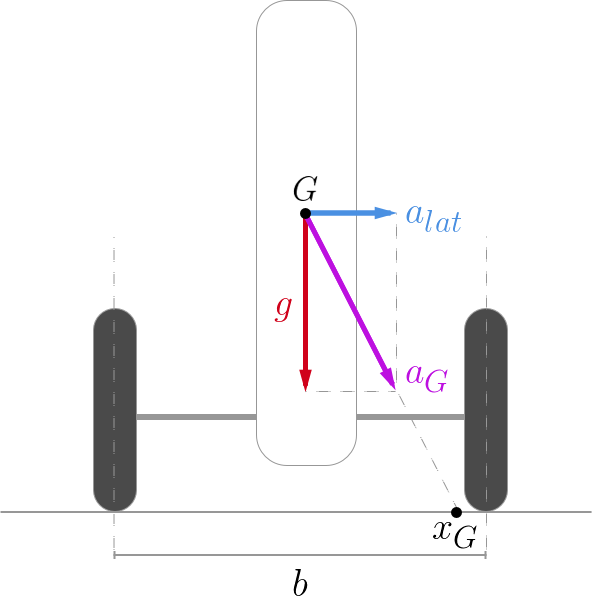
\includegraphics[width=1.2\linewidth]{figs/03/stability}
	\caption{Forces acting on the center of gravity}
	\label{stability}
\end{marginfigure}
In this section the dynamics of the vehicle are examined from the expression of $a_{per}$, in three distinct cases: 
\begin{enumerate}
\item \textbf{Vertical vehicle in straight path}

In this case $\theta=0$ and $a_{lat}=0$, therefore $a_{per}=0$ and the problem of lateral stability does not arise, except for the cases of rejection of lateral disturbance forces (i.e. side winds), or disturbances due to an asymmetric pavement on the left and right wheels. 

\item \textbf{Vertical vehicle in circular trajectory}

When the vehicle does not tilt (i.e $\theta=0$), then $a_{per}=a_{lat}$ (see equation (\ref{a_per})). If the intersection of the resultant accelerations at the center of gravity $G$ with the plane of the ground (point $x_G$) is outside the base of the vehicle, then it will be unstable. 
\[a_{G}=a_{lat}\,\vec{j} -g\,\vec{k}\]
On the contrary, if the point $x_G$ recalls inside the width of the vehicle, it will be stable. Then, the maximum lateral acceleration tolerated without inclination before the overturn is:
\begin{equation}
a_{lat-max}=\frac{gb}{2h}
\end{equation}
\\[-1cm]
\item \textbf{Inclined vehicle in circular trajectory}

When the vehicle is inclined at a certain angle $\theta$, its center of gravity has an offset, as well as the point $x_G$. The vehicle is stable as long as $x_G$ belongs to the segment $b$ and is, therefore, located between the two wheels of the vehicle. Let $\theta_n$ be the nominal inclination angle for which all accelerations in G are compensated, so that is solution of $a_{per}=0$. The computation of $\theta_n$ can seem complicated, but by considering the steady state (i.e. $\ddot{\theta}=\dot{\theta}=0$): $a_{per}=a_{lat}\cos\theta-g\sin\theta$. We then deduce the following expression:
\[\theta_{ref}=\theta_{n}=\tan^{-1}\Big(\frac{a_{lat}}{g}\Big)\]
This angle gives a resultant $a_{G}$ colinear with the axis $z'$ of the vehicle. Thus, the angle $\theta_{n}$ (solution of $a_{per}=0$) is an angle that guarantees the lateral stability of the vehicle.
\end{enumerate}

\subsection{Different strategies for lateral control}

The objective is to control the inclination of the vehicle so as to ensure its stability. In this way, the lateral stability of the vehicle and the comfort of passengers go hand in hand. From the sufficient condition of the stability explained above, the way to achieve this is by having null perceived acceleration at the center of gravity, $a_{per}=0$.

Two control strategies can be followed to reach this objective:

\begin{enumerate}
\item The stability is ensured by a \textbf{direct angular position control}, considering the angle of inclination of reference $\theta_{ref}$ ensuring $a_{per}=0$. This strategy has been widely adopted by researchers working on this issue. However, this strategy has some drawbacks: approximations have to be made to obtain at each moment the adapted reference angle, and its calculation potentially induces a \textbf{delay in the control}. 

\item An alternative solution is to \textbf{directly control the perceived acceleration}, and to pursue the $a_{per}=0$ objective. This is the strategy followed in this thesis. 
\end{enumerate}

Provided that the most readily available measurements on the vehicle are those provided by an inertial unit (IMU), the choice of direct control of $a_{per}$ was better adapted for these sensors.

\section{State of the Art for DTC, STC and SDTC systems}
Having defined the vehicle model, explained the problem of lateral stability, and calculated the various quantities concerned (lateral acceleration, perceived acceleration) it is now possible to clearly explain the work and results obtained by different researchers.

\begin{itemize}
\begin{itemize}
	\item \textbf{Hibbard Robbin \textit{et al.} 1996}\cite{hibbard1996twenty}, considered the problem of DTC vehicles and proposed to control the angle of inclination with the value of the reference calculated according to $\theta_{ref}$. The lateral acceleration was approximated by $V_{x}\dot{\psi}$, ignoring the dependence in $\ddot{y}$
\[\theta_{ref}=\tan^{-1}\Big(\frac{a_{lat}}{g}\Big)=\tan^{-1}\Big(\frac{\ddot{y}+V_{x}\dot{\psi}}{g}\Big)\approx\frac{V_{x}\dot{\psi}}{g}\] The control used for position feedback was a Proportional Derivative (PD) that has the error input on $\theta$, $e=\theta-\theta_{ref}$ with a feedforward function $a_{lat}=V_{x}\doc{\psi}$. The model used for regulator adjustment was reduced to the simplified transfer function between $\theta$ and $M_t$.

\item \textbf{So S. \textit{et al.}, 1997a}\cite{doi:10.1080/00423119708969321}, were interested in a system where STC and DTC actuated alternately, depending on the longitudinal speed of the vehicle.
\begin{itemize}
\item A filtered PD regulator was used for the DTC system: \[M_{t}=\Big(K_{p}+\frac{K_{d}}{\tau_{1}s+1}\Big)(\theta-\theta_{ref})\]
\item The STC strategy similarly used a PD with filtered derivative to calculate the appropriate steering angle.
\item The authors exploited the approximate relationship between $a_{lat}$ and $\delta$: $a_{lat}=\ddot{y}+V\dot{\psi}=(\dot{V}\,L_{r}\,\delta+V\,L_{r}\,\dot{\delta}+V^{2}\delta)/(L_{f}+L_{r})$. So $\theta_{ref-STC}=a_{lat}/g=f(\delta,\dot{\delta})$ and the control signal STC is written: \[\delta=\Big(G_{p}+\frac{G_{d}s}{\tau_{2}s+1}\Big)(\theta-\theta_{ref-STC})\]
\item The two controllers were first simulated separately, considering only the simplified transfer functions between $\delta$ and $\theta$ in STC and between the tilt torque $M_t$ and $\theta$ for DTC. The proposed results showed that the perceived acceleration in DTC was much greater than in STC, and that at the same time the steering angle was significantly modified in STC; 
\item Switching between STC and DTC systems was also considered, at speeds of $7.5 m/s$ and $8.5m/s$ depending on a hysteresis cycle. To circumvent the jump problems with respect to the static control value, the authors proposed a variable gain for the STC, which increased gradually to optimal value.
\end{itemize}

\item In their work, \textbf{So S. \textit{et al.}, (1997)}\cite{doi:10.1504/IJVD.1997.062071} replaced the PD controller with a PI for the DTC system to solve the static error problem and minimize discontinuity during STC-DTC switching. They added an additional feedback gain as a function of $\theta$ and $\dot{\theta}$. 

The validation of this work was very basic since no stability study was available, the lateral $a_{lat}$ and perceived $a_{per}$ accelerations were reconstructed by their approximate mathematical expressions and were not supposed to be directly measured; The simulations were carried out on a simplified model, linearized around $\theta=0$, considering the lateral and longitudinal dynamics.
\newpage
\item At the University of Minneapolis, the researchers addressed several aspects of lateral control of narrow tilting vehicles. In their work, \textbf{Piyabongkran D. \textit{et al.} (2004)}\cite{piyabongkarn2004active}, proposed three DTC control strategies in order to control the angle of inclination at $\theta_{ref}=\tan^{-1}(V\dot{\psi}/g)$, based on the linearized lateral model. 

\begin{itemize}
\item The first strategy was based on a Linear Quadratic Regulator (LQR) using a simplified model whose states only corresponded to $\theta$ and $\dot{\theta}$, hence ignoring the coupling with other important variables such as the yaw rate $\dot{\psi}$. A model of the driver was implemented to correct errors on the trajectory in simulation. 
\item The second strategy was based on the LQR control with a predictive aspect provided by the predictive estimation of the reference inclination angle, based on the knowledge of the future trajectory (i.e. on-board camera, GPS, etc. thus predicting the curvature of the road). The reference angle was obtained through a predictive command with a Receding Horizon Controller. 
\item The third proposed control strategy was nonlinear; it proceeded by inversion of the dynamics of the inclination angle (linearization by looping), which resulted in a double integrator dynamics $M_{t}=\ddot{\theta}$. A PID was then used such that $M_{t}=(K_{p}+K_{d}s+K_{i}/s)(\theta-\theta_{ref})$ 
\end{itemize}

The simulations showed that the nonlinear controller (strategy 3) was much more efficient than the LQ controller (strategy 2) in minimizing the tilt torque. The best performances were nevertheless obtained with the RCH controller (strategy 2), underlining the importance of the anticipation of the transient performance of the inclination control.

\item The SDTC commands were discussed by \textbf{Kidane, S. \textit{et al.} (2008), (2010})\cite{doi:10.1080/00423110701352987,5356230}. The authors proposed 3 DTC strategies, and 3 STC strategies, in order to find the methodology ensuring the best switching in SDTC. 

The \textbf{DTC strategies} were all based on a PD controller, but differed in the expression of the reference $\theta_{ref}$ chosen:
\begin{enumerate}
\item $\theta_{ref}=\frac{V\dot{\psi}}{g}=\frac{V^2}{gR}$
\item $\theta_{ref}=\frac{\ddot{y}+V\dot{\psi}}{g}-\frac{2(I_{wheel rot}\,w\,\dot{\psi}/(hm)}{g}$
\item $\theta_{ref}=k_{s}(\delta_{driver})$
\end{enumerate}

The first expression is the most simplified; it neglects the term of lateral slip $\ddot{y}$, which leads to a significant increase in the transient torque. The second expression is more rigorous and the term $2(I_{wheel rot}\,w\,\dot{\psi}/(mgh)$, which takes into account the gyroscopic moments at the level of the wheels, leads to a zero static error, but it is difficult to calculate. Finally, to circumvent the problem of contradictory STC and DTC control signals, the authors retained the third expression (i.e. $\theta_{des}=k_{s}(\delta_{driver})$), although it is very approximate and does not optimize the torque required in transient situations. 

The \textbf{STC strategies} also used a PD controller, with an additional term $\delta_{ss}$, which allowed a steering angle equal to that desired by the driver to be obtained in steady state: $\delta=K_{p}(\theta-\theta_{ref})+K_d{\dot{\theta}-\dot{\theta}_{ref})+\delta_{ss}$. The three STC strategies differed in their choice of $\delta_{ss}$:

\begin{enumerate}
\item The most complete proposed expression uses the value of unmeasured and therefore inaccessible variables.
\item An alternative expression performs the rewriting of expression 1. as a function of $\theta_{ref}$ and parameters to be estimated.
\item The last strategy replaces $\delta_{ss}$ by an integral term on the deviation $(\theta-\theta_{ref})$. This is the solution chosen for the SDTC command.
\end{enumerate}

\item The \textbf{SDTC controller} was then made up of two independent PIDs; one controller generated the motor torque $M_{t}$, and the second the steering angle $\delta$ applied to the wheels. $V_o$ and $V_f$ were two threshold values, $V_{o}<V_{f}$ for the longitudinal velocity. For $V<V_{o}$, the DTC system is active; for $V>V_{f}$, the STC system takes over; For $V_{o}<V<V_{f}$ a function dependent on $V$ shared the control between DTC and STC. 

The controller was validated in simulation and experimentally by \textbf{Kidane S. \textit{et al.}, 2010}\cite{5356230}. The results were acceptable, but the perceived lateral acceleration was not given, and no stability study was proposed. On the other hand, the proposed SDTC controller did not explicitly optimize the energy required for implementing this strategy.
\newpage

\item In the Netherlands, \textbf{Carver Europe} developed a three-wheel recliner called Carver. This vehicle was equipped with a Dynamic Vehicle Control system that used the DTC and STC strategies. The publications relating to this system remain evasive, probably due to the confidentiality of the project. However, several patents are filed separately concerning the use of the steering angle in the tilt controller (CR Van Den Brink \textit{et al.}, 1999)\cite[-3cm]{van1999realization}, the simultaneous action of the STC and DTC systems (CR Van Den Brink And Kroonen, 2004)\cite{van1997dynamic}.

\item At the \textbf{University of Bath}, researchers worked on the \textbf{Clever} project: a three-wheeled vehicle, in which only the chassis and front wheel were tilted. This vehicle was equipped with a DTC system, operating with hydraulic actuators. In their work, Berote \textit{et al.}, (2008)\cite{bath15090} the authors focused on the analysis of the Clever dynamics, emphasizing the importance of rear wheel steering to limit the risk of over-turning of the vehicle. The authors also evoked the advantage of having the axis of rotation of the vehicle inclined (and not horizontal), which affects the inertia of the inclination movement. The DTC controller remained very basic: a PD to control the angle of inclination. 

\end{itemize}
\end{itemize}

\newpage
\section{DTC: Summary of Difficulties and Solutions}

In this section the problems of DTC control are identified, and solutions are proposed to improve the performance of the controller.

\subsection{Difficulties related to DTC} 

DTC strategies are generally based on a pursue of the angle of inclination $\theta$, such that $\theta\rightarrow\theta_{ref}$, where $\theta_{ref}$ is given by the expression  $\theta_{ref}=\tan^{-1}(a_{lat}/g)$ or even more simplified or approximate versions which have been described in detail in the previous section (i.e. $\theta_{ref}=V_{x}\dot{\psi}/g$, or $\theta_{ref}=k_{s}(\delta_{driver})$, etc.). The weak points of these strategies can be summarized as follows:
\begin{enumerate}
\item \textbf{High torque from the actuator on the transient phase}: the calculation of $\theta_{ref}$ from the measurement of lateral acceleration $a_{lat}$ or yaw angle $\dot{\psi}$, induces an \textbf{intrinsic delay}: the actuator is only activated after the detection of the lateral acceleration through the accelerometer. The inclination torque must therefore compensate for the lateral acceleration already present, which inclines the vehicle towards the outside of the curve before being able to incline it in the opposite direction with the actuator. 

\begin{figure*}[!h]
	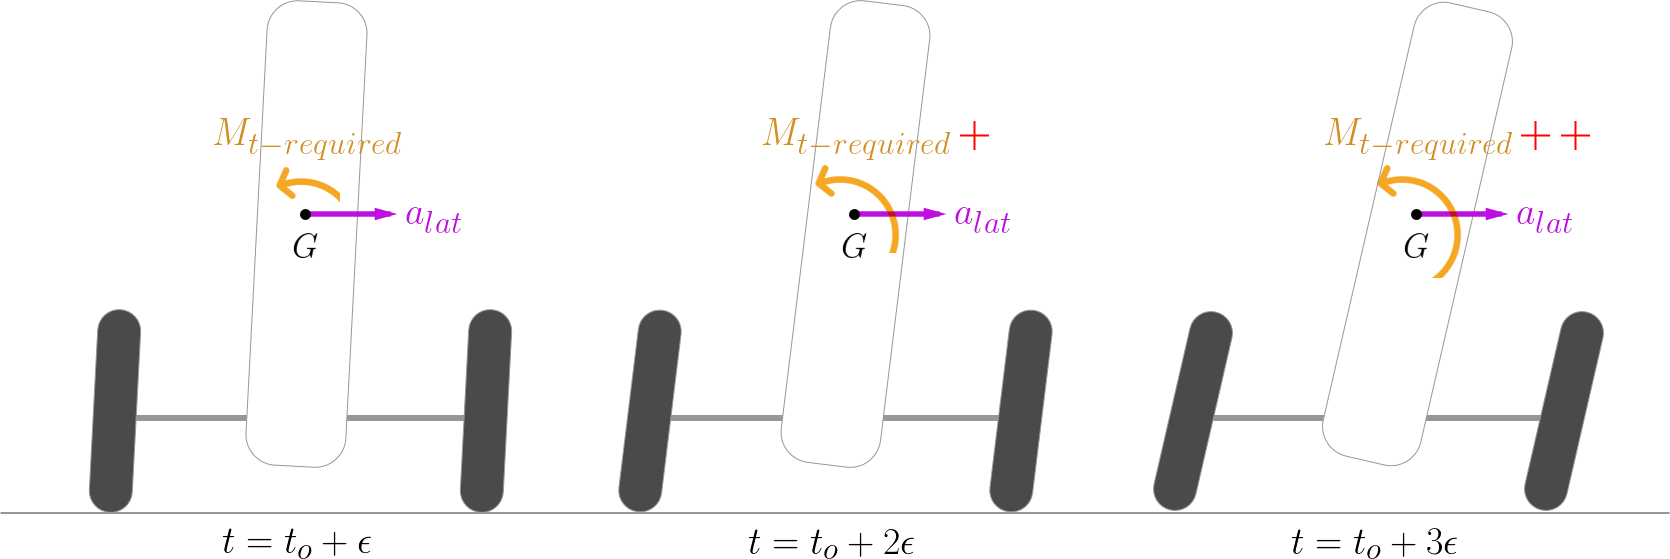
\includegraphics[width=1.0\linewidth]{figs/03/torque}
	\caption{Transitional phase of the vehicle approaching a turn: increasing $a_{lat}$, inclining the vehicle outside the turn and requiring a greater $M_t$}
	\label{torque}
\end{figure*}

The longer the $M_t$ reaction, the greater the lateral acceleration, and the greater the required tilt torque. When other sensors that allow the trajectory prediction are installed on the vehicle (camera), this anticipation makes it possible to reduce the tilting torque significantly (Piyabongkran D. and Al., 2004)\cite[0cm]{piyabongkarn2004active}. In addition, the lateral acceleration ($a_{lat}=\ddot{y}+V\dot{\psi}\cos\beta$) is proportional to the speed. Thus, the higher the speed, the greater the lateral acceleration and the greater the torque $M_t$ required.
\newpage
\item \textbf{Static error}: Given the way in which the reference is calculated,  $\theta=\theta_{ref}$ does not mean that $a_{per}$ is strictly null. Consequently, the actuator must permanently supply a non-zero torque to maintain the inclination of the vehicle at $\theta_{ref}$.
\end{enumerate}
\subsection{Proposed solutions} 

The two main solutions to improve the operation of the DTC systems are: A) Using the steering angle input from the driver as a regulator and B) Directly controlling the perceived lateral acceleration.
\begin{enumerate}
\item \textbf{Reduction of the actuator torque in DTC}

When driving of a motorcycle, the rider tilts it as soon as the turn begins, before the appearance of the lateral acceleration. Consequently the effort required for the inclination is relatively small; and this is also the case for a vehicle whose path is known in advance. It is, thus, essential to initiate the inclination as soon as possible. 

The first measurable signal containing information about the near trajectory is the \textbf{angle (or even the torque) of steering}. This signal must be used in order to initiate the inclination of the vehicle before the perception of lateral acceleration. %This will be an essential part of the strategy followed in this thesis.

The steering angle is considered as a \textbf{disturbance} which induces an increase in the perceived lateral acceleration, such as to destabilize the vehicle. In order to be able to use this signal in the controller, a control methodology is chosen to be able to take into account this knowledge of the environment. 

\item \textbf{Cancellation of the static error and improvement of the DTC performance}

The lateral stability is obtained by the appropriate inclination of the vehicle. It is therefore intuitive to seek to control the angle of inclination $\theta\rightarrow\theta_{ref}$ by calculating the necessary torque to achieve an inclination coherent with the terminal objective: $a_{per}=0$. To reduce the problem of the approximation and to reduce the risks of instability ($\theta_{ref}$ is deduced from the state variables) the \textbf{direct control of the perceived lateral acceleration} $a_{per}$ is proposed.\cite{6315042}

Therefore, the objective variable is now the $a_{per}=0$ rather than $\theta=\theta_{ref}$. In addition, in order to ensure the robust asymptotic cancellation of the static error, the integral of $a_{per}$ ($a_{per}^{I}$) will be taken into account. This approach is much more interesting since $a_{per}$ is measured by the inertial motion unit (IMU).
\end{enumerate}
\newpage
\section{Design of the DTC Controller}
\subsection{Dynamic Model}
In the previous chapter, the linearized dynamic model was obtained:
\begin{eqnarray}
\label{dynamic_model_1}
m\ddot{y}+mV \dot{\psi}+mh\ddot{\theta}=F_{f}+F_{r} \\
I_{z}\,\ddot{\psi}=L_{f}F_{f}-L_{r}L_{r}-(I_{wr,\theta}-I_{wr,rot})w_{rot}\dot{\theta}-M_{\delta}\\
I_{x} \ddot{\theta}=mgh\theta -F_{f}h-F_{r}h + +2(I_{wf,\psi}-I_{wf,rot})w_{rot}(\dot{\psi}+\dot{\delta}) +M_{t}\\
2\,I_{wf,\psi}\ddot{\delta}=M_{\delta}+M_{trail}-2(I_{wf,\theta}-I_{wf,rot})w_{rot}\dot{\theta}
\label{dynamic_model_2}
\end{eqnarray}
\[F_{f}=2 C_{f}\Big(\delta - \frac{\dot{y}+L_{f} \dot{\psi}}{V} \Big) + 2 \lambda_{f} \theta\]
\[F_{r}=C_{r}\Big(- \frac{\dot{y}-L_{r} \dot{\psi}}{V} \Big) +\lambda_{r} \theta\]

The inputs to this model are the steering angle $\delta$ and the tilting torque $M_{t}$.

\subsection{Methodological Approach}
The general idea consists in formalizing the problem through the construction of a generic model, called standard, allowing the reformulation of the problem of control in an optimization problem $H_{2}$\cite[-2cm]{Zhou:1996:ROC:225507}. This model $P(S)$ is structured and consists of the aggregation of:
\begin{itemize}
\begin{itemize}
\item \textbf{Plant}: A model of the system to be monitored, displaying disturbance and control signals and well as the output variables to be controlled.
\item \textbf{Disturbance}: A model of the environment of the system to be controlled, generating the exogenous signals such as perturbations and setpoints.
\item \textbf{Output}: A model of the quantities to be regulated, including weights constituting adjustment coefficients.
\end{itemize}
\end{itemize}
\begin{marginfigure}[-4.5cm]
	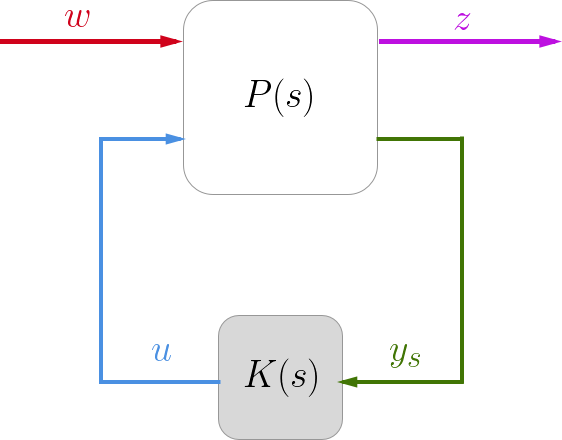
\includegraphics[width=1.2\linewidth]{figs/03/standard}
	\caption{Standard Problem}
	\label{standard}
\end{marginfigure}

The associated $H_{2}$ is considered in the generic form, which consists in determining $K_{s}$ stabilizing the process model and minimizing: $\lVert P(s)\,K(s) \rVert _{2}$

\subsection{State Space Model}
The obtained model of the form described by equations (\ref{dynamic_model_1}-\ref{dynamic_model_2}) is reduced to its controllable and observable part which has 4 states $(\dot{y},\dot{\psi},\theta,\dot{\theta})$.
The Linear Parameter Variant (LTV) model is parameterized by the longitudinal speed $V$ of the vehicle:
%\begin{equation}
%\begin{cases}\dot{x}(t)=A(V)\,x(t)+B\,u(t)\\ y(t)=C\,x(t)+D\,u(t)\end{cases}
%\end{equation}
\begin{equation}
\begin{cases}\dot{x}=A\,x+B_{u}\,u+B_{d}\,d\\ y=C\,x+D_{u}\,u+D_{d}\,d\end{cases}
\end{equation}

with $x^{T}=\begin{bmatrix}
\dot{y} & \dot{\psi} & \theta & \dot{\theta}
\end{bmatrix}^{T} \in \Re^4$, $u=M_{t}$ and $d=\delta$

$A=\begin{bmatrix} 
\frac{1}{V}\big(-\frac{a}{m}-\frac{h^{2}a}{I_{x}}\big) & \frac{1}{V}\big(-\frac{b}{m}-\frac{h^{2}b}{I_{x}}\big)-V & (2\lambda_{f}+\lambda_{r})\big(\frac{1}{m}+\frac{h^2}{I_{x}}\big)-\frac{mgh^2}{I_{x}} & 0\\
-\frac{b}{V\,I_{z}} & -\frac{2C_{f}L_{f}^{2}+C_{r}L_{r}^{2}}{V\,I_{z}} & \frac{2\lambda_{f}L_{f}-\lambda_{r}L_{r}}{I_{z}} & 0\\
0 & 0 & 0 & 1\\
\frac{h\,a}{V\,I_{x}} & \frac{h\,b}{V\,I_{x}} & \frac{mgh-h(2\lambda_{f}+\lambda_{r}}{I_{x}} & 0
\end{bmatrix}
$\\[10pt]
$B_{d}=B_{\delta}=\begin{bmatrix} 2C_{f}\big(\frac{1}{m}+\frac{h^2}{I_{x}} & \frac{2C_{f}L_{f}}{I_{z}} & 0 & -\frac{2C_{f}h}{I_{x}} \end{bmatrix}^{T}$,\\[10pt]
$B_{u}=B_{M_{t}}=\begin{bmatrix} -\frac{h}{I_{x}} & 0 & 0 & \frac{1}{I_{x}} \end{bmatrix}^{T}$, $a=2\,C_{f}+C_{r}$, $b=2\,C_{f}L_{f}-C_{r}L_{r}$

The model becomes an Linear Time Invariant (LTI) model when a constant longitudinal velocity $V$ is considered. The vector $x$ denotes the states , $y$ the measured the outputs, $u$ the control input and $d$ is considered as a disturbing exogenous signal\cite{kCraig}.

\subsection{Estimation of $\dot{y}$}
The PEV will include a Inertial Measurement Unit (IMU), which will provide the state values $\theta$, $\dot{\theta}$, and $\dot{\psi}$, but not $\dot{y}$. The IMU will also give the value for the perceived lateral acceleration $a_{per}$. Note that this measure was not used in the previous strategy, nor in the classical strategy of controlling $\theta$ such that $\theta=\theta_{des}$ steering angle $\delta$ and its derivative $\dot{\delta}$ will be measured.

The state signal $\dot{y}$ can be estimated from the measured signals: $y_{p}=\begin{bmatrix}
\dot{\psi} & \theta & \dot{\theta} & a_{per} \end{bmatrix}^{T}$, according to:\\[8pt]
\begin{aligned}
\hat{\dot{y}}=(a_{11}+ha_{41})^{-1}\Big[a_{per}-(a_{12}+ha_{42}+V_{x})\dot{\psi}-(a_{13}+ha_{43}-g)\theta \\- (a_{14}+ha_{44})\dot{\theta}-(b_{\delta 1}+hb_{\delta 4})\delta-(b_{u1}+hb_{u4})M_{t}\Big]
\end{aligned}
\\[8pt] where terms $a_{ij}$, $b_{\delta i}$ and $b_{ui}$ are coefficients of matrices $A$, $B_{\delta}$ and $B_{u}$ respectively.

\subsection{Expressing $a_{per}$ as function of $x$}
Lateral stability of the vehicle is obtained when the sum of lateral forces and torques at its center of gravity is zero ($a_{per}=0$). 

$\hspace{1.5cm} a_{per}=a_{lat}\cos\theta+h\ddot{\theta}-g\sin\theta$\quad with  \quad $a_{lat}=\ddot{y}+V\,\dot{\psi}$

The $a_{per}$ is a measured signal, but is not part of the state vector. Using small angle approximations, it can be expressed as a function of the state vector as follows:
\[a_{per}\approx\ddot{y}+V\,\dot{\psi}+h\ddot{\theta}-g\theta=a_{per}^{lin}\]
\[a_{per}^{lin}=\begin{bmatrix} 0 & V & -g & 0 \end{bmatrix} x + \begin{bmatrix} 1 & 0 & 0 & h \end{bmatrix} \dot{x}=G_{1}\,x+G_{2}\,\dot{x}\]

Replacing $\dot{x}$ by $A\,x+B_{u}\,u+B_{d}\,d$ leads to:
\[a_{per}^{lin}=G_{1}\,x+G_{2}(A\,x+B_{u}\,u+B_{d}\,d)=G\,x+H_{u}\,u+H_{d}\,d\]
with $G=G_{1}+G_{2}\,A$, $H_{u}=G_{2}\,B_{u}$ and $H_{d}=G_{2}\,B_{d}$. The output vector is defined as $y=\begin{bmatrix} a_{per} & \dot{\psi} & \theta & \dot{\theta} & \delta \end{bmatrix}^{T}$ Therefore:

$\hspace{2cm} C=\begin{bmatrix}
G \\ \begin{bmatrix} 0_{3x1} I_{3} \end{bmatrix} \\ 0_{1x4} 
\end{bmatrix}$, $D_{u}=\begin{bmatrix}
H_{u} \\ 0_{4x1}
\end{bmatrix}$, $D_{d}=\begin{bmatrix}
H_{d} \\ 0_{3x1} \\ 1
\end{bmatrix}$

\subsection{Regulator Problem with Internal Stability \cite{6315042}}

The fundamental control objective to ensure the lateral stability is to solve the regulation problem $a_{per}=0$. The problem formulation is recast as a standard regulator problem with internal stability (RPIS) where $\delta$ is considered as a disturbance, and its effect on the perceived lateral acceleration $a_{per}$ should be canceled by the tilt torque $M_{t}$. 

\begin{figure}[!h]
	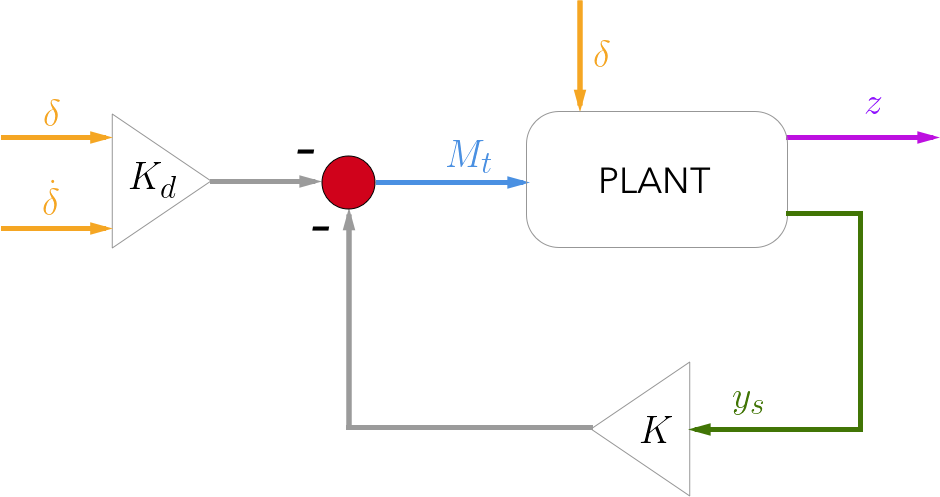
\includegraphics[width=0.95\linewidth]{figs/03/control}
	\caption{Control diagram: Feedforward and feedback loops}
	\label{control}
\end{figure}

\textbf{Plant Model}
\begin{equation}
\begin{cases}\dot{x}=A\,x+B_{u}\,u+B_{d}\,d\\ y=C\,x+D_{u}\,u+D_{d}\,d\\ z=G\,x+H_{u}\,u+H_{d}\,d\end{cases}
\end{equation}
with $G=\begin{bmatrix}
-{a}/{V\,m} & -{b}/{V\,m} & (2\lambda_{f}+\lambda_{r})/m - g & 0
\end{bmatrix} \\[6pt] H_{u}=0, H_{d}={2C_{f}}/{m}$

\textbf{Disturbance Model} 
\begin{equation}
\begin{cases}\dot{x_{e}}=A_{e}\,x+B_{e}\,w\\ d=C_{e}\,x_{e}\end{cases}
\end{equation}
with $x_{e}^{T}=\begin{bmatrix}
\delta & \dot{\delta}
\end{bmatrix}^{T}$, $C_{e}=\begin{bmatrix}
1 & 0
\end{bmatrix} $, $A_{e}=\begin{bmatrix}
0 & 1 \\ -\tau\alpha & -(\tau +\alpha) 
\end{bmatrix}$, $B_{e}=\begin{bmatrix}
0 \\ \beta
\end{bmatrix}$

where $w$ is an impulse signal, $\alpha$, $\tau$ and $\beta$ determine the time constants and amplitude of the $2^{nd}$ order signal. This model is critical to obtain good performances in transient phases, while the feedback takes care of the static ones and guarantees robust regulation.

\textbf{Standard Model}\\[6pt]
\[\begin{bmatrix} \dot{x} \\ \dot{x_{e}} \end{bmatrix} = \begin{bmatrix}
A & B_{d}\,C_{e} \\ 0 & A_{e}\end{bmatrix}\begin{bmatrix} x \\ x_{e} \end{bmatrix} +\begin{bmatrix} B_{u} \\ 0 \end{bmatrix} u + \begin{bmatrix}0 \\ B_{e} \end{bmatrix} w\]

\[e=z=\begin{bmatrix}G & H_{d}\,C_{e}\end{bmatrix}\begin{bmatrix}x \\ x_{e}\end{bmatrix} + H_{u}\,u\]

\[y=\begin{bmatrix}x \\ x_{e}\end{bmatrix}=\begin{bmatrix}
\dot{y} & \dot{\psi} & \theta & \dot{\theta} & \delta & \dot{\delta}\end{bmatrix}^{T}\]

\textbf{Solution for RPIS}

Assuming that the plant model is stabilizable, a solution for the RPIS problem exists in the feedback form if the unique solution ($T_{a},F_{a}$) of the occultation equations exists:
\begin{eqnarray}
-A\,T_{a}+T_{a}\,A_{e}+B_{d}\,C_{e}=-B_{u}\,F_{a} \\
-G\,T_{a}+H_{d}\,C_{e}=H_{u}\,F_{a}
\end{eqnarray}

If $\exists\, T_{a}, F_{a} \rightarrow u_{ref}=-F_{a}\,x_{e}$ and $x_{ref}=-T_{a}\,x_{e}$ is the unique reference trajectory for the plant model that satisfies the control objective $e=a_{per}=0$. Therefore this trajectory satisfies the dynamic of the system:
\begin{equation}
\begin{cases}\dot{x}_{ref}=A\,x_{ref}+B_{u}\,u_{ref}+B_{d}\,d\\ z_{ref}=G\,x_{ref}+H_{u}\,u_{ref}+H_{d}\,d\end{cases}
\label{sylvester}
\end{equation}
Defining $(\tilde{u},\,\tilde{x},\,e)=(u-u_{ref},\,x-x_{ref},\,z-z_{ref})$ the difference between the actual and desired values of the current control input, states and controlled output.

The first step is to compute the feedback gain $K$, designed such that $\tilde{u}=-K\tilde{x}$ guarantees $\tilde{x}\rightarrow 0$ and $e\rightarrow 0$ (stabilization of the plant). The second step a feedforward gain is designed in order for $(u,x)$ to follow the reference trajectory $u_{ref},x_{ref}$ in an optimal way.

\textbf{Feedback Gains}

For the calculation of the feedback gains, the Linear Quadratic Regulator (LQR)\cite{lec5}\cite{rob3}\cite{Wonham:1614618} has been chosen based on the good robustness properties, few tuning parameters and the explicit minimization of the energy of control signals required to follow the reference.

The LQR consists on finding the state feedback $\tilde{u}=-K\tilde{x}$ that minimizes the criteria:
\[J_{LQR}=\int_{0}^{\infty}{\big(z^{T}\,Q\,z + u^{T}\,R\,u \big) dt}=\int_{0}^{\infty}{\big(x^{T}\,Q_{x}\,x + u^{T}\,R\,u + 2 x^{T}\,N_{xu}\,u\big) dt}\]
The weighting matrices $Q$ and $R$ must be positive and will balance the minimization of the state vector or the control signal.
\[Q_{x}=G^{T}\,Q\,G\]
\[R_{u}=H_{u}^{T}\,Q\,H_{u} + R\]
\[N_{ux}=G^{T}\,Q\,H_{u}\]
The solution is given by:
\[K=-R_{u}^{-1}\,B_{u}^{T}\,P\]
Where $P$ is the unique solution of the Riccati equation applied to the plant model:
\[A^{T}\,P+P\,A-P\,B_{u}\,R_{u}^{-1}\,B_{u}^{T}\,P+Q_{x}=0\]

\textbf{Feedforward Gains}

Solving the Sylvester equations in (\ref{sylvester}) and using the feedback gains $K$, the feedforward gain is calculated as $K_{d}=F_{a}+K\,T_{a}$.

\begin{aligned}
\tilde{u}=-K\tilde{x} \quad \rightarrow \quad & u-u_{ref}=-K\,(x-x_{ref}) \\[6pt] & u + F_{a}\,x_{e}=-K(x+T_{a}\,x_{e} \\
& u=-K\,x -(F_{a}+K\,T_{a})x_{e}=-K\,x-K_{d}\,x_{e}
\end{aligned}

\subsection{Extended model with the integral of $a_{per}$: $a_{per}^_{I}$}
In order to avoid any static error, the integrated value of the lateral perceived acceleration will be controlled, and its value will be added to the state vector. In fact, it is unavoidable to have some model errors due to parameters uncertainty, neglected dynamics or linearization of the model.

The equation to add to the model is very simple: 
\[\dot{a_{per}^_{I}}=a_{per}=G\,x+H_{u}\,u+H_{d}\,d\]
The augmented state is then $x_{i}=\begin{bmatrix} \dot{y} & \dot{\psi} & \theta & \dot{\theta} & a_{per}^_{I} \end{bmatrix}$, and the new system:
\begin{equation}
\begin{cases}\dot{x_{i}}=A\,x_{i}+B_{iu}\,u+B_{id}\,d\\ z=a_{per}^_{I}}=G_{i}\,x_{i}+H_{iu}\,u+H_{id}\,d\end{cases}
\end{equation}

\[A_{i}=\begin{bmatrix} A & 0_{4x1} \\ G & 0{1x1} \end{bmatrix}, \quad B_{iu}=\begin{bmatrix} B_{u} \\ H_{u} \end{bmatrix}, \quad B_{id}=\begin{bmatrix} B_{d} \\ H_{d} \end{bmatrix}\]
\[G_{i}=\begin{bmatrix} 0 & 0 & 0 & 0 & 1 \end{bmatrix}, \quad H_{iu}=0, \quad H_{id}=0\]

\textbf{Extended Standard Model}\\[6pt]
\[\begin{bmatrix} \dot{x_i} \\ \dot{x_{e}} \end{bmatrix} = \begin{bmatrix}
A_{i} & B_{id}\,C_{e} \\ 0_{2x5} & A_{e}\end{bmatrix}\begin{bmatrix} x_{i} \\ x_{e} \end{bmatrix} +\begin{bmatrix} B_{iu} \\ 0_{2x1} \end{bmatrix} u + \begin{bmatrix}0_{2x1} \\ B_{e} \end{bmatrix} w\]\\[6pt]
\[e=z=a_{per}^_{I}}=\begin{bmatrix}G_{i} & H_{id}\,C_{e}\end{bmatrix}\begin{bmatrix}x_{i} \\ x_{e}\end{bmatrix} + H_{iu}\,u\]\
\[y=\begin{bmatrix}x \\ x_{e}\end{bmatrix}=\begin{bmatrix}
\dot{y} & \dot{\psi} & \theta & \dot{\theta} & a_{per}^_{I} & \delta & \dot{\delta}\end{bmatrix}^{T}\]

\textbf{Feedback Gains}

The Linear Quadratic Regulator is adapted to the extended model: 
\[J_{LQR}=\int_{0}^{\infty}{\big(z^{T}\,Q\,z + u^{T}\,R\,u \big) dt}=\int_{0}^{\infty}{\big(x^{T}\,Q_{x}\,x + u^{T}\,R\,u + 2 x^{T}\,N_{xu}\,u\big) dt}\]
\[Q_{x}=G_{i}^{T}\,Q\,G_{i} \hspace{1cm} R_{u}=H_{iu}^{T}\,Q\,H_{iu} + R \hspace{1cm} N_{ux}=G_{i}^{T}\,Q\,H_{iu}\]
The solution is given by:
\[K=-R_{u}^{-1}\,B_{iu}^{T}\,P\]
Where $P$ is the unique solution of the Riccati equation applied to the plant model:
\[A_{i}^{T}\,P+P\,A_{i}-P\,B_{iu}\,R_{u}^{-1}\,B_{iu}^{T}\,P+Q_{x}=0\]

\textbf{Feedforward Gains}

The Sylvester equations in (\ref{sylvester}) need to be adapted to the new model:
\begin{eqnarray}
-A_{i}\,T_{a}+T_{a}\,A_{e}+B_{id}\,C_{e}=-B_{iu}\,F_{a} \\
-G_{i}\,T_{a}+H_{id}\,C_{e}=H_{iu}\,F_{a}
\end{eqnarray}
By solving these equations and using the feedback gains $K$, the feedforward gain is calculated as $K_{d}=F_{a}+K\,T_{a}$.

\textbf{Simple Method Gains Calculation}

A straightforward way of calculating the gains is to solve the Riccati and the Sylvester equations as it is indicated in (Friedland, Chapter 9.6)\cite{control-system-design} book:

	-- Riccati eq: $\quad M_{1}\,A_{i} + A_{i}^{T}\,M_{1} - M_{1}\,B_{iu}\,R_{u}^{-1}B_{iu}^{T}M_{1} + Q_{x}=0$

	-- Slyvester eq: $\quad M_{2}\,A_{e}+(A_{i}^{T}-M_{1}\,B_{iu}\,R_{u}^{-1}\,B_{iu}^{T})M_{2}+M_{1}\,B_{id}\,C_{e}=0$

Then, the gains can be easily calculated:
\begin{itemize}
\begin{itemize}
\item Feedback gains: $K=R_{u}^{-1}\,B_{iu}^{T}\,M_{1}$
\item Feedforward gains: $K_{d}=R_{u}^{-1}\,B_{iu}^{T}\,M_{2}$
\end{itemize}
\end{itemize}

\subsection{Derivation of the Gains}

As was discussed previously, the state variable $\dot{y}$ is not measured and can only be estimated as:

\begin{aligned}
\hat{\dot{y}}=(a_{11}+ha_{41})^{-1}\Big[a_{per}-(a_{12}+ha_{42}+V_{x})\dot{\psi}-(a_{13}+ha_{43}-g)\theta \\- (a_{14}+ha_{44})\dot{\theta}-(b_{\delta 1}+hb_{\delta 4})\delta-(b_{u1}+hb_{u4})M_{t}\Big]
\end{aligned}

To calculate the real gains on the controller, a simple but tedious derivation has to be carry out:
\[u=-K\,x_{i}-K_{e}\,x_{e}\]
\[u=-K_{\dot{y}}\,\dot{y}-K_{\dot{\psi}}\,\dot{\psi}-K_{\theta}\,\theta-K_{\dot{\theta}}\,\dot{\theta}-K_{a_{per}^{I}}\,a_{per}^{I}-K_{\delta}\,\delta-K_{\dot{\delta}}\,\dot{\delta}\]
\newpage
\begin{aligned}
u&=-\frac{K_{\dot{y}}}{a_{11}+ha_{41}}\,a_{per} - \Big(K_{\dot{\psi}}-K_{\dot{y}}\frac{a_{12}+ha_{42}+V_{x}}{a_{11}+ha_{41}}\Big)\dot{\psi} -  \Big(K_{\theta}-K_{\dot{y}}\frac{a_{13}+ha_{43}-g}{a_{11}+ha_{41}}\Big)\theta - \Big(K_{\dot{\theta}}-K_{\dot{y}}\frac{a_{14}+ha_{44}}{a_{11}+ha_{41}}\Big)\dot{\theta} - \\[10pt] &\quad -  K_{a_{per}^{I}}\,a_{per}^{I} - \Big(K_{\delta}-K_{\dot{y}}\frac{b_{\delta 1}+hb_{\delta 4}}{a_{11}+ha_{41}}\Big)\delta-K_{\dot{\delta}}\,\dot{\delta}-K_{\dot{y}}\,\frac{b_{u1}+hb_{u4}}{a_{11}+ha_{41}}\,u
\end{aligned}
\\

\begin{aligned}
u=\frac{1}{1+K_{\dot{y}}\,\frac{b_{u1}+hb_{u4}}{a_{11}+ha_{41}}}\Big[&-\frac{K_{\dot{y}}}{a_{11}+ha_{41}}\,a_{per} - \Big(K_{\dot{\psi}}-K_{\dot{y}}\frac{a_{12}+ha_{42}+V_{x}}{a_{11}+ha_{41}}\Big)\dot{\psi} - \Big(K_{\theta}-K_{\dot{y}}\frac{a_{13}+ha_{43}-g}{a_{11}+ha_{41}}\Big)\theta - \\[10pt] & - \Big(K_{\dot{\theta}}-K_{\dot{y}}\frac{a_{14}+ha_{44}}{a_{11}+ha_{41}}\Big)\dot{\theta} -  K_{a_{per}^{I}}\,a_{per}^{I} - \Big(K_{\delta}-K_{\dot{y}}\frac{b_{\delta 1}+hb_{\delta 4}}{a_{11}+ha_{41}}\Big)\delta-K_{\dot{\delta}}\,\dot{\delta}\Big]
\end{aligned}
\\

\begin{aligned}
u=\frac{1}{a_{11}+ha_{41}+K_{\dot{y}}\,(b_{u1}+hb_{u4})}\Big[&-K_{\dot{y}}\,a_{per} - \big[K_{\dot{\psi}}(a_{11}+ha_{41})-K_{\dot{y}}(a_{12}+ha_{42}+V_{x})\big]\dot{\psi} - \\[8pt] & - \big[K_{\theta}(a_{11}+ha_{41})-K_{\dot{y}}(a_{13}+ha_{43}-g)\big]\theta - \\[8pt] & - \big[K_{\dot{\theta}}(a_{11}+ha_{41})-K_{\dot{y}}(a_{14}+ha_{44})\big]\dot{\theta} -  K_{a_{per}^{I}}(a_{11}+ha_{41})\,a_{per}^{I} - \\[8pt] & - \big[K_{\delta}(a_{11}+ha_{41})-K_{\dot{y}}(b_{\delta 1}+hb_{\delta 4})\big]\delta-K_{\dot{\delta}}(a_{11}+ha_{41})\,\dot{\delta}\Big]
\end{aligned}
\\

With this estimation all the signals are measured and have a gain:
\begin{eqnarray}
K_{a_{per}}^{'}=\frac{K_{\dot{y}}}{a_{11}+ha_{41}+K_{\dot{y}}\,(b_{u1}+hb_{u4})} \\[10pt]
K_{\dot{\psi}}^{'}=\frac{K_{\dot{\psi}}(a_{11}+ha_{41})-K_{\dot{y}}(a_{12}+ha_{42}+V_{x})}{a_{11}+ha_{41}+K_{\dot{y}}\,(b_{u1}+hb_{u4})} \\[10pt]
K_{\theta}^{'}=\frac{K_{\theta}(a_{11}+ha_{41})-K_{\dot{y}}(a_{13}+ha_{43}-g)}{a_{11}+ha_{41}+K_{\dot{y}}\,(b_{u1}+hb_{u4})} \\[10pt]
K_{\dot{\theta}}^{'}=\frac{K_{\dot{\theta}}(a_{11}+ha_{41})-K_{\dot{y}}(a_{14}+ha_{44})}{a_{11}+ha_{41}+K_{\dot{y}}\,(b_{u1}+hb_{u4})} \\[10pt]
K_{a_{per}^{I}}^{'}=\frac{K_{a_{per}^{I}}(a_{11}+ha_{41})}{a_{11}+ha_{41}+K_{\dot{y}}\,(b_{u1}+hb_{u4})} \\[10pt]
K_{\delta}^{'}=\frac{K_{\delta}(a_{11}+ha_{41})-K_{\dot{y}}(b_{\delta 1}+hb_{\delta 4})}{a_{11}+ha_{41}+K_{\dot{y}}\,(b_{u1}+hb_{u4})} \\[10pt]
K_{\dot{\delta}}^{'}=\frac{K_{\dot{\delta}}(a_{11}+ha_{41})}{a_{11}+ha_{41}+K_{\dot{y}}\,(b_{u1}+hb_{u4})}
\end{eqnarray}
\[K^{'}=\begin{bmatrix}
K_{a_{per}}^{'} & K_{\dot{\psi}}^{'} & K_{\theta}^{'} & K_{\dot{\theta}}^{'} & K_{a_{per}^{I}}^{'} & K_{\delta}^{'} & K_{\dot{\delta}}^{'}
\end{bmatrix} \]
\newpage
\subsection{Gain Scheduled Controller}
The previous regulator was synthesized by considering a constant value of the longitudinal speed $V_{x}$. But the state space model is LPV and the matrices $A$ and $C$ depend on $V$ or $1/V$. Thus, the proposed controller is not valid for the whole speed range. In this section, a controller that depends on the longitudinal speed of the vehicle is proposed. 

The approach adopted is pragmatic, and proceeds by interpolation of the LTI regulators obtained for a discrete set of longitudinal speeds. It thus guarantees a good performance at every operating point. Stability guarantees will also be provided by a posteriori analysis. 

The first step is the observation of the gain variation of this regulator as a function of velocity for $V \in {2,3,...18}\,m/s $. A regulator is synthesized for each value of $V$ and the variation of the gains can be approximated by a function of the form:
\[K(V)=K_{c}+K_{V}\,V+K_{1/V)\V\]
Dependent on $V$ and $1/V$, with $K_{c}$, $K_{V}$ and $K_{1/V}$ the constants to be identified. These values can be easily deduced from the least squares resolution of the following system of equations:
\[
\underbrace{\begin{pmatrix}
1 & V_{1} & 1/V_{1} \\ 1 & V_{2} & 1/V_{2} \\ ... & ... & ... \\ 1 & V_{17} & 1/V_{17} \\
\end{pmatrix}}_{M} 
\begin{pmatrix} K_{c} \\ K_{V} \\ K_{1/V} \end{pmatrix}=
\underbrace{\begin{pmatrix} K_{V_{1}}^{'} \\K_{V_{2}}^{'} \\ ... \\ K_{V_{17}}^{'} \end{pmatrix}}_{K_{M}}
\Rightarrow
\begin{pmatrix} K_{c} \\ K_{V} \\ K_{1/V} \end{pmatrix}=(M^{T}\,M)^{-1}\,M^{T}\,K_{M}\]

\newpage
\section{Control Strategy Summary}
In this chapter the control strategy has been completely derived and developed. The process of calculating the gains can be resumed in few steps:
\begin{enumerate}
\item To obtain or measure the \textbf{parameters to complete the dynamic model}. This includes the vehicle and the wheels variables: 

$\hspace{2cm} m \enspace L_{f} \enspace L_{r} \enspace I_{x} \enspace I_{z} \enspace C_{f} \enspace C_{r} \enspace \lambda_{f} \enspace \lambda_{r} \enspace ...$.

\item To suppose a \textbf{constant $V$ for the model}, so that $V \in {2,3,...18}\,m/s $

\item To generate the \textbf{matrices of the state space} model:

$\hspace{1.5cm} A \enspace B_{u} \enspace B_{d} \enspace C \enspace D_{u} \enspace D_{d} \enspace G \enspace H_{u} \enspace H_{d} \enspace A_{e} \enspace B_{e} \enspace C_{e} \enspace ...$

\item \textbf{Feedback gains}: To solve the Riccati equation for the selected model and calculate the gains: 

$\hspace{1.5cm} M_{1}\,A_{i} + A_{i}^{T}\,M_{1} - M_{1}\,B_{iu}\,R_{u}^{-1}B_{iu}^{T}M_{1} + Q_{x}=0$

$\hspace{3.5cm} K=R_{u}^{-1}\,B_{iu}^{T}\,M_{1}$

\item \textbf{Feedforward gains}: To solve the Slyvester equation for the selected model and calculate the gains: 

$\hspace{1cm}M_{2}\,A_{e}+(A_{i}^{T}-M_{1}\,B_{iu}\,R_{u}^{-1}\,B_{iu}^{T})M_{2}+M_{1}\,B_{id}\,C_{e}=0$

$\hspace{3.5cm} K_{d}=R_{u}^{-1}\,B_{iu}^{T}\,M_{2}$

\item \textbf{Gain Scheduling}: To repeat the steps 2 to 5 with all the speed range and calculate the constants $K_{c}$, $K_{V}$ and $K_{1/V}$  with:

$\hspace{2.5cm}\begin{pmatrix} K_{c} \\ K_{V} \\ K_{1/V} \end{pmatrix}=(M^{T}\,M)^{-1}\,M^{T}\,K_{M}$

\end{enumerate}
